% Use only LaTeX2e, calling the article.cls class and 12-point type.

\documentclass[12pt]{report}
\usepackage[a4paper]{geometry}
\usepackage[myheadings]{fullpage}
\usepackage{fancyhdr}
\usepackage{lastpage}
\usepackage{graphicx, wrapfig, subcaption, setspace, booktabs}
\usepackage[T1]{fontenc}
\usepackage[font=small, labelfont=bf]{caption}
\usepackage{fourier}
\usepackage[protrusion=true, expansion=true]{microtype}
\usepackage[english]{babel}
\usepackage{sectsty}
\usepackage{url, lipsum}
\usepackage{tgbonum}
\usepackage{hyperref}
\usepackage{xcolor}

\pagestyle{fancy}
\setlength\headheight{15pt}
\fancyhead[L]{Student ID: 40076898}
\fancyhead[R]{Concordia University}


% Users of the {thebibliography} environment or BibTeX should use the
% scicite.sty package, downloadable from *Science* at
% www.sciencemag.org/about/authors/prep/TeX_help/ .
% This package should properly format in-text
% reference calls and reference-list numbers.



% Use times if you have the font installed; otherwise, comment out the
% following line.

\usepackage{times}

% The preamble here sets up a lot of new/revised commands and
% environments.  It's annoying, but please do *not* try to strip these
% out into a separate .sty file (which could lead to the loss of some
% information when we convert the file to other formats).  Instead, keep
% them in the preamble of your main LaTeX source file.


% The following parameters seem to provide a reasonable page setup.

\topmargin 0.0cm
\oddsidemargin 0.1cm
\textwidth 16cm 
\textheight 22cm
\footskip 1.0cm


%The next command sets up an environment for the abstract to your paper.

\newenvironment{sciabstract}{%
\begin{quote} \bf}
{\end{quote}}




% If your reference list includes text notes as well as references,
% include the following line; otherwise, comment it out.

\renewcommand\refname{References and Notes}

% The following lines set up an environment for the last note in the
% reference list, which commonly includes acknowledgments of funding,
% help, etc.  It's intended for users of BibTeX or the {thebibliography}
% environment.  Users who are hand-coding their references at the end
% using a list environment such as {enumerate} can simply add another
% item at the end, and it will be numbered automatically.

\newcounter{lastnote}
\newenvironment{scilastnote}{%
\setcounter{lastnote}{\value{enumiv}}%
\addtocounter{lastnote}{+1}%
\begin{list}%
{\arabic{lastnote}.}
{\setlength{\leftmargin}{.22in}}
{\setlength{\labelsep}{.5em}}}
{\end{list}}


% Include your paper's title here

\title{The Universal Parabolic Constant\\ \textbf{Eternity Numbers}}
\date{2018\\ July}
\author{By Ali Zafar Iqbal\\\\ Department of Computer Science \\Concordia University }

% Include the date 
\date{}
\begin{document} 
\maketitle 
\titleformat{\subsection}{\small\bfseries}

% Double-space the manuscript.

\baselineskip20pt

% Make the title.

% Place your abstract within the special {sciabstract} environment.
\tableofcontents


\graphicspath{ {./Universal Parabolic Constant Mindmap/}{./images2/} }



\newpage




  \chapter{Introduction}
  
  The primary focus of this project is an exploratory study of a unique irrational constant (The Universal Parabolic Constant), its use in society and finally its structured implementation process. this project document will confer a through analysis about the number's comprehensive background and its implementation process into its unique form of calculator.
  \section{Intro into Irrational Numbers }
    An irrational number is a number that cannot be expressed as a fraction p/q for any integers p and q. Irrational numbers have decimal expansions that neither terminate nor become periodic.s
\section{Universal parabolic constant}
   \\
    
     The Universal Parabolic Constant  is a type of irrational number[3] , its defined as the ratio, for any parabola or Semicircle, of the arc length of the parabolic segment formed by the Latus-rectum to the focal parameter (Two time the focal length), it is donated by the Constant letter "P" According to Revolvy [1] the circle parabolas are unique among conic sections and hence have a universal constant where as ellipses and hyperbolas do not.
     
    
    \begin{equation}
    {P=\ln(1+{\sqrt {2}})+{\sqrt {2}}=2.29558714939\dots }
    \end{equation}
 
 \section{Properties and Derivation}
\\
 P is described to be a  "Transcendental number", which when elaborated upon are real/complex numbers that are not a root of a nonzero polynomial equation. according to many online sources [1][3] its characteristics are much more in line with "Pi" however it has a more monotonous/specific function in practice. Its derivation is as follows.
\begin{enumerate}



    \begin{equation}
    
    {\displaystyle {P&:={\frac {1}{p}}\int _{-\ell }^{\ell }{\sqrt {1+\left({\frac {dy}{dx}}\right)^{2}}}
    \end{equation}
    
    \begin{equation}
    
    {dx&={\frac {1}{2f}}\int _{-2f}^{2f}{\sqrt {1+{\frac {x^{2}}{4f^{2}}}}}\,dx\\&=\int _{-1}^{1}{\sqrt {1+t^{2}}}\,dt\quad (x=2ft)\\&=\operatorname 

    \end{equation}
    
    \begin{equation}
    ={arcsinh} (1)+{\sqrt {2}}\\&=\ln(1+{\sqrt {2}})+{\sqrt {2}}}}
    \end{equation}

\end{enumerate}
\hfill\\
 \section{Applications}
 \\
According to online documentation [3], Universal Parabolic Constant can be used to calculate the \average distance from a random point in the square unit to the center of the parabola. This can be used to measure practical distances during the constitution of real world objects such as Satellite Dishes where Incoming waves are concentrated on a singular focal point. Or architectural arcs where the extreme of arcs may need accurate points of measurements for their constructions 

 \begin{equation}
{d_{\text{avg}}={P \over 6}.}
 \end{equation}


 



 \chapter{Concept Exploration}
 
 
 \section{Mindmapping and Viability analysis}
 
 As evident from the start of the project, time was a precious commodity during the duration of this project therefore to avoid redundancy of work, an extensive Mindmap was drawn out to understand the eventual goal of the project as well as the structure the contents to be presented in this report, possible user bases were explored using the mind map to compare and contrast the best possible users to focus on and ultimately interview within the duration of the week. \\
 
 \noindent Furthermore, The mind map also allowed to explore the possible use cases of the assigned constant before a full through diagram could be drawn out for it.

  \begin{figure}
    \subsection{Project Mindmap}
     \centering
     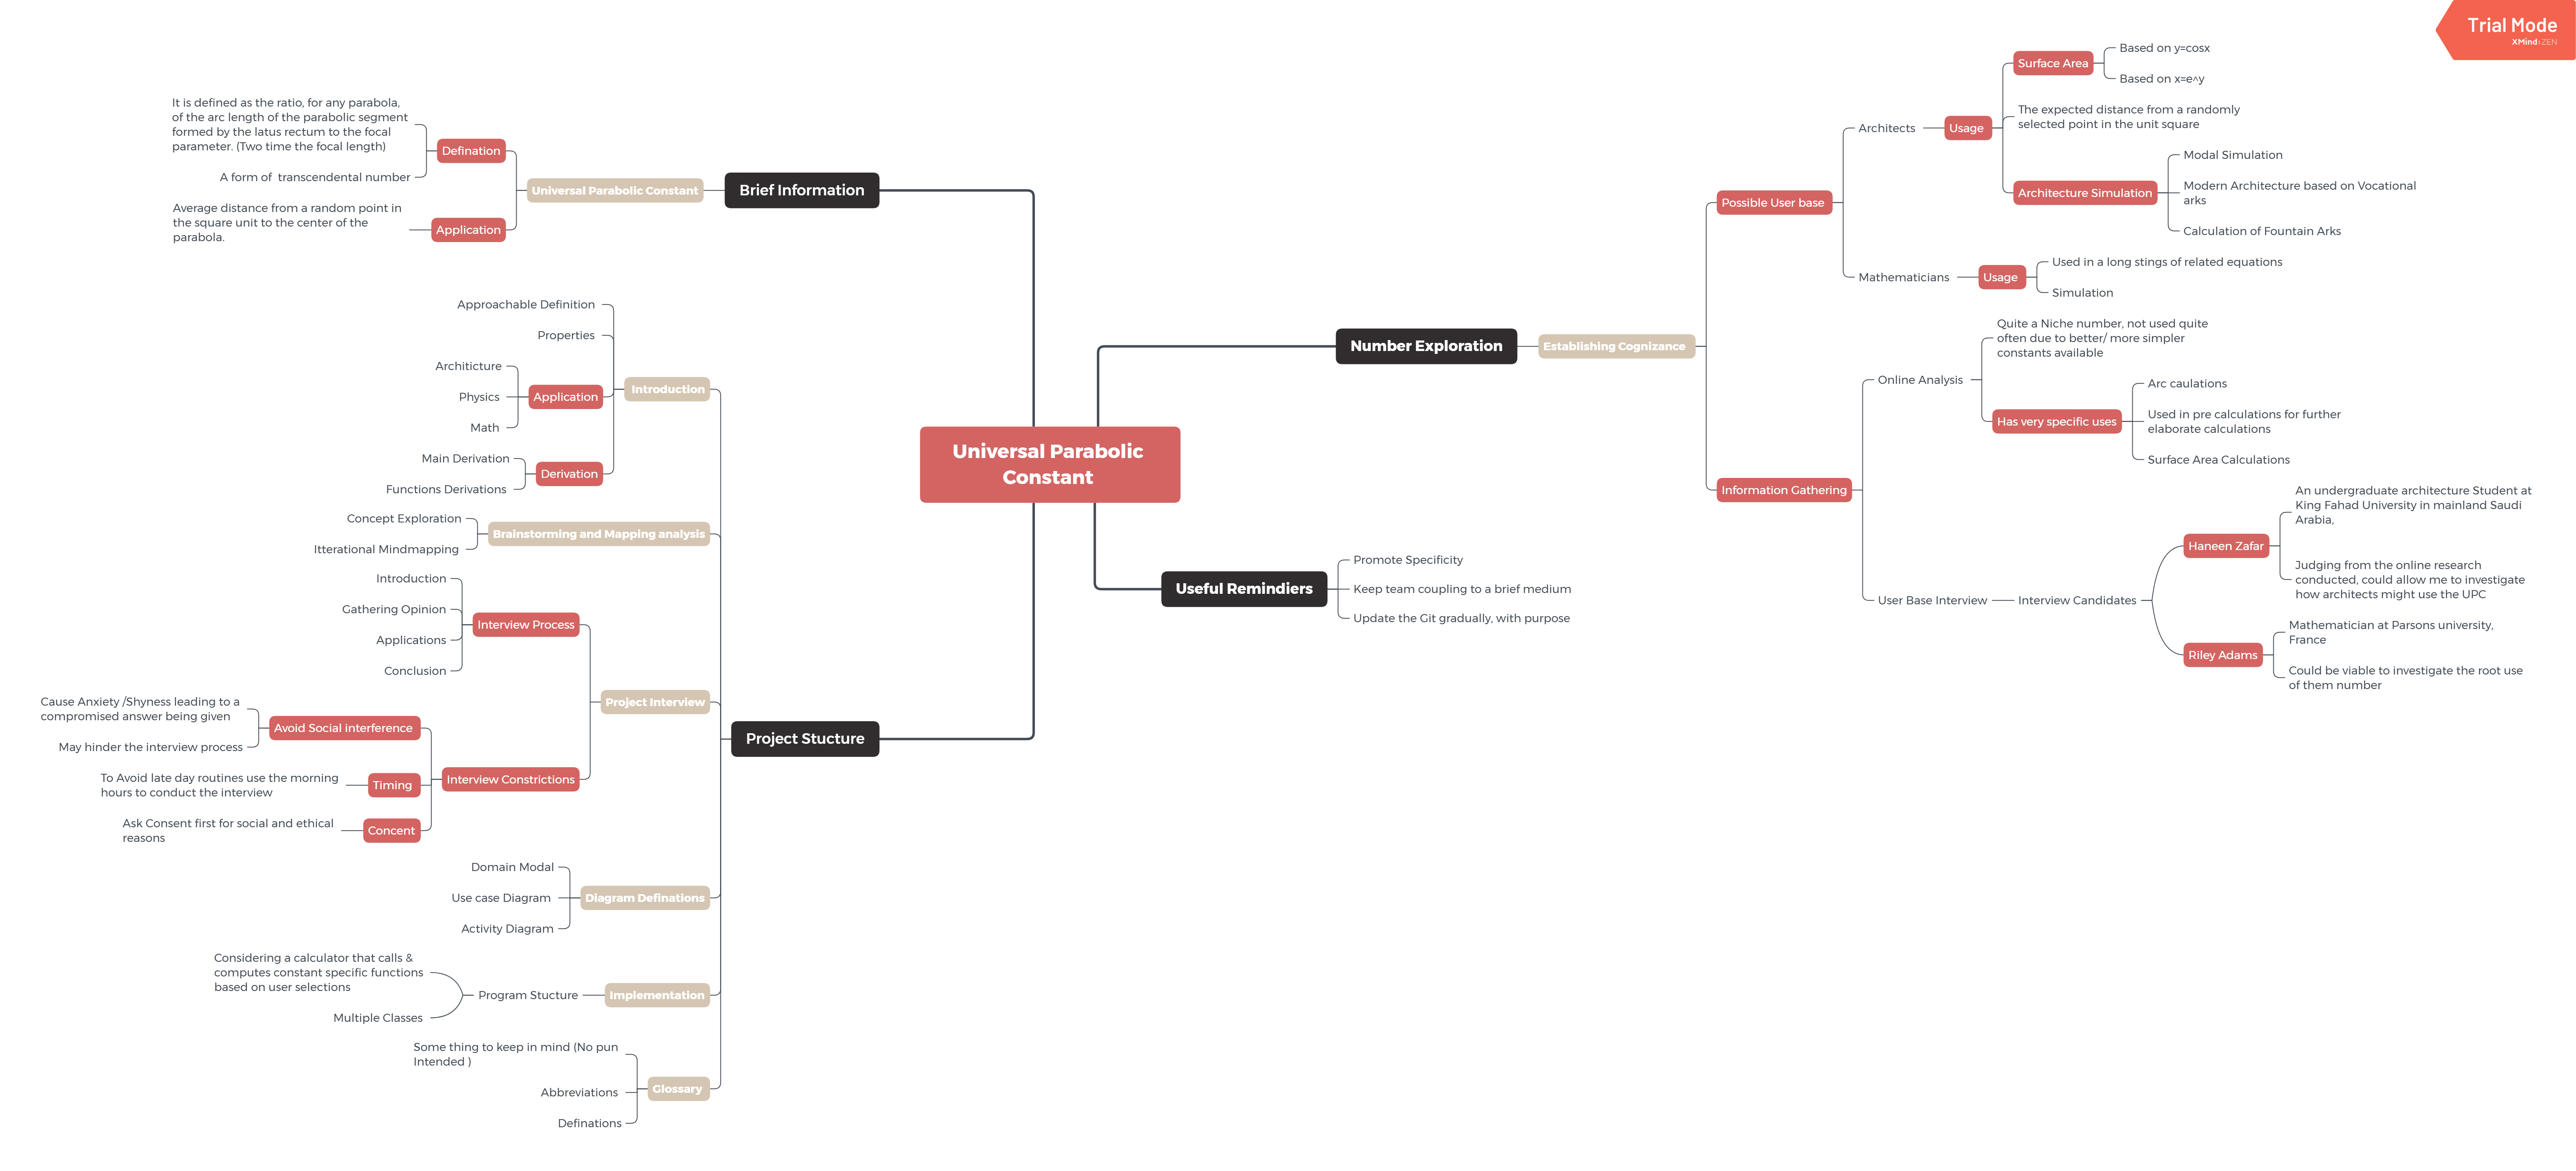
\includegraphics[width=\textwidth]{Assets/Mindmap.png}
     \caption{Project Mindmap for the Universal Parabolic Constant}
     \label{fig:my_label}
 \end{figure}




\chapter{Project Interview}



\begin{flushleft}

Apart from a documentation exploration of my problem domain about Eternity Number, an exploratory interview was conducted for the creation of this report to understand the need of the Universal parabolic constant in practical environment and how laymen people come about to actually use the mathematical constant on a day to day basis.   
\newpage

  \begin{figure}
  \section{User Personification}
\noindent \addlinespace Before approaching possible candidates for the interview, a generalized user persona was drawn out detailing an explicit background and biological information to help the investigative process of finding a suitable interview candidate.\hfill\\

     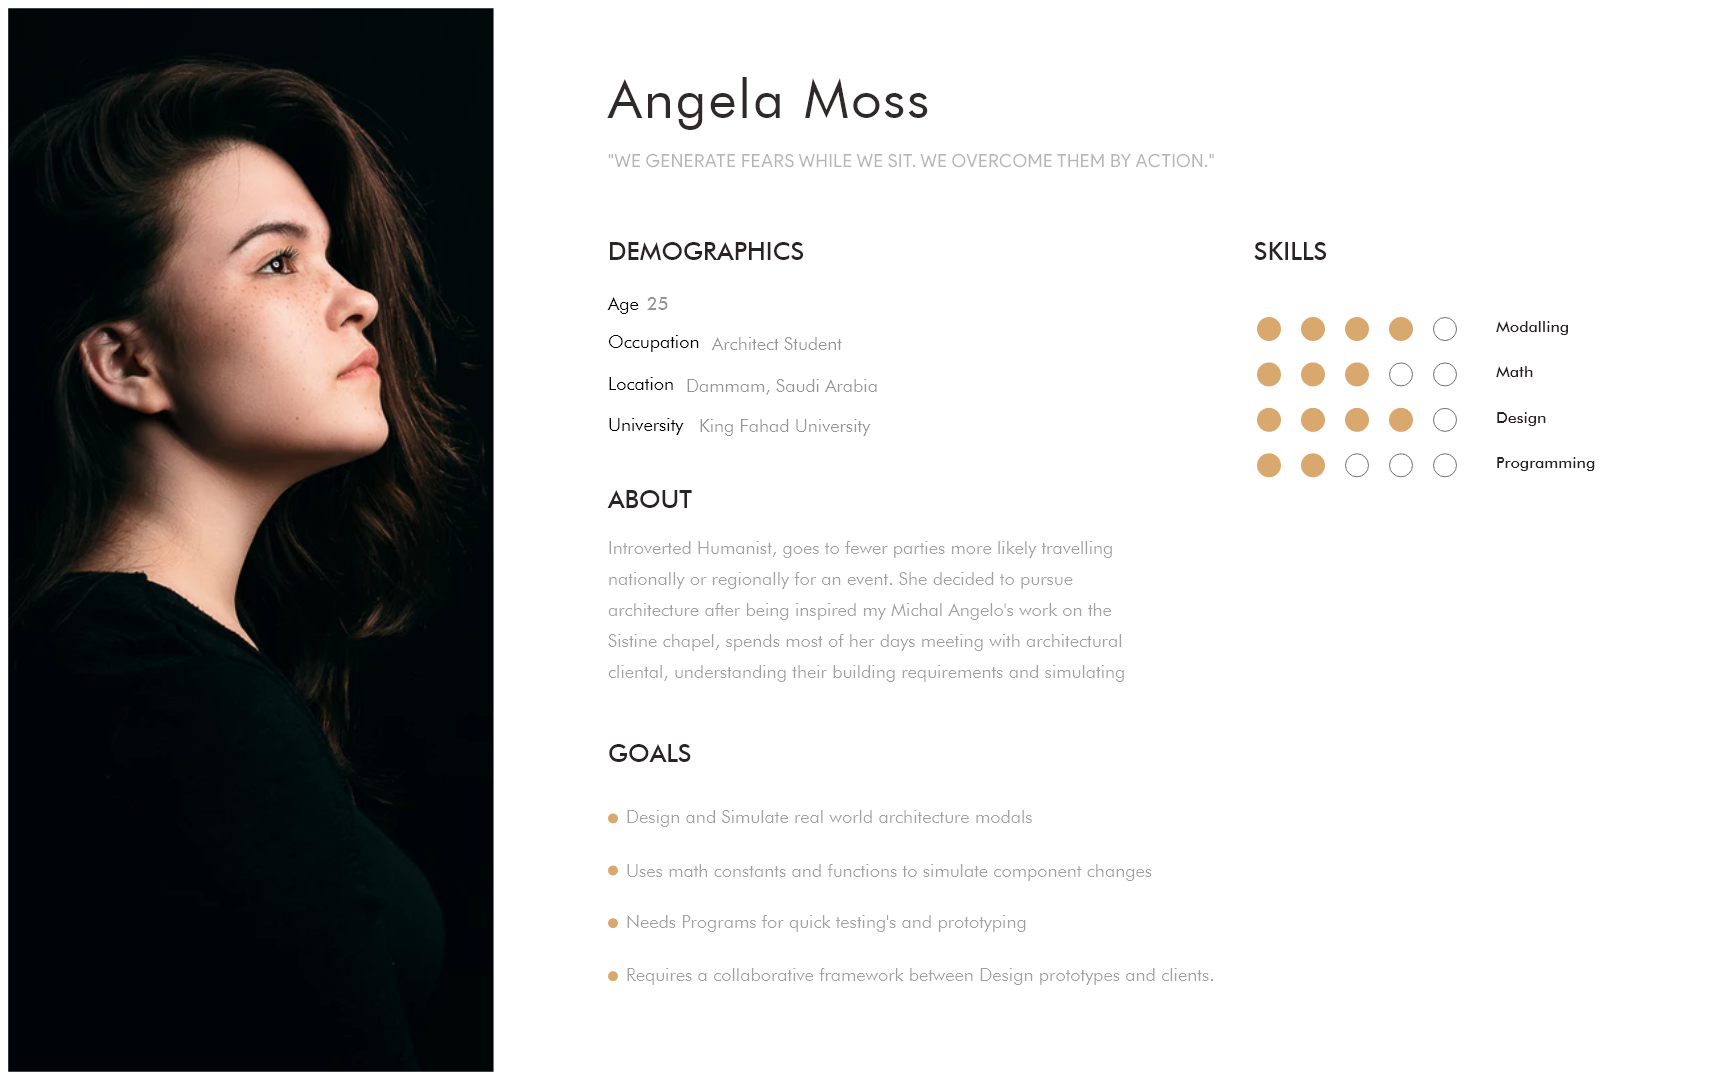
\includegraphics[width= \textwidth]{Assets/UserPersona.png}
     \caption{User Persona}
     \label{fig:my_label}
 \end{figure}
 \newpage
\section{Subject Background}

 The Interviewee subject selected for the project is \textbf{Haneen Zafar}, an undergraduate architecture Student at King Fahad University in mainland Saudi Arabia, Studying architecture in her final years of university, she was found to be a suitable candidate for interview section of the exploratory study of the Universal Parabolic constant in light to its extensive use in the field of architecture simulations and arc based calculations. \\
\section{Interview Constraints}

The interview was conducted in an isolated room environment over a phone call, to allow the subject to be calm and free to answer during the interviewing process, this was done to eliminate any sources of hesitation or social anxiety that may occur during the interviewing . The Interview was Started around 10:30 AM in the morning EST and lasted around 15 Mins excluding the conclusion.
\section{Interview Structure}
To pragmatic value of the report and to enable conformity of documentation process, the interview was structured into 4 Parts, with the individual parts labeled as follows.
\begin{enumerate}

\item{Introduction}
\item{Domain Consciences}
\item{Applications of the Constant}
\item{Conclusion}
\end{enumerate}

\subsection{Introduction}

To make the interviewee feel relaxed and welcomed, this section featured an initial set of questions focused understanding the hierarchical persona of the person  \hfill \break

   \begin{quote}
       
   
    \textbf{1. Please State your name and vocation for the purposes of the  interview ?}
    
    Answer : Hi Ali, My name is Haneen, I am an Architectural student currently in my final year of study in King Fahad University in Saudi Arabia.  
    \hfill \break
   
    \textbf{2. Can you elaborate on your field of study in University?}
    
    Answer : I study mostly architectural works and construct modal concepts both physically and in software systems to simulate possible structures with real world constructs realized.
    \hfill \break 
    
    \textbf{3. Your work in architecture was one of the reasons I contacted you for this interview, I wanted to inquire , how often do you use Mathematical Constants in your studies/work? }
    
    Answer : Heh, I am sure you know that any forms of  buildings cannot be realized without a certain degree of mathematical knowledge. So yes we do use constants in our works. Like Pi, Golden ratios etc. but to be honest with you,  I rely on my trusty rulers quite more heh. 
    \hfill \break
    \end{quote} 
    
    
    
    \subsection{Domain Consciences (Understanding the Constant/ Problem Domain)}
    
    The section of the Interview focused on getting information about the Universal parabolic constant and to diagnose how well the interviewee is familiar with the subject.
     \hfill 
    \begin{quote}
    \textbf{4. For my university project, I am supposed to figure out certain applications for a mathematical constant, are you familiar with the Universal Parabolic constant?}
    
    Answer : Yes actually It was thought to us in one of our classes here at the university, \hfill \break
   
    \textbf{5. Oh Nice, so In your opinion What uses do architects find with this constant? }
    
    Answer : Heh, you'd be surprised, honestly I mean as the name states, Parabolas are used everywhere in Architecture, from Suspension bridges , Fountains  to modern art structures. The constant allows us to proximate distances of possible structural degradation/changes over time, this can be because of let's say Gravity or  differences caused by changes in environmental temperatures. \hfill \break
    \end {quote}
    
    \subsection{Applications of the Number}
 This sections had incremental questions to the topic's root, focused more on understanding the ideal use cases of the number in a architectural environment  
     \hfill \break

     \begin {quote}
    \textbf{6. How often and in what areas do you find yourself using the Universal Parabolic Constant?}
    
    Answer : Like I said it depends, mostly for our approximations we pre simulate our structural diagrams in blender or 3D Max for presentation purposes, however like the example I gave you, when you are calculating stuff like structural changes caused by heat you need to use approximation constants like the UPC combined with various other functions to calculate the differences in distances from median before and after the change. even the area or circular structure, but under very specific circumstances. \hfill \break
   
    \textbf{7. So Imagine, If an application was developed, what forms of functions would you like to perform with the constant?}
    
    Answer : Answer : Hmm, It would be nice if I could combine my pre existing functions to your Parabolic constant, Like we do on an actual calculator, but on the top of my head, I can't think of any heh. \hfill \break
     \end {quote}
    \subsection{Conclusion}

   The section of the Interview focused on debriefing the subject, and getting their consent on using the information obtained during the interviewing process for the purposes of this project. \hfill \break

    \begin {quote}
    \textbf{8. Thanks for your time Haneen, You can't Imagine how helpful your insights are to my project.}
    
    Answer : Oh, it was no problem,just the time difference was a bit of trouble on my end, as you can imagine I have classes \hfill \break

    \textbf{9. Yes, Apologies for that, I have a short work notice for my project, So time is something that is fleeting to me. May I contact you again If I am in need of further insights for my project? }
    
    Answer : Sure, Just be sure to let me know beforehand, as It would allow me to adjust my schedule for your call.\hfill \break
    \end {quote}
    \subsection{Interview analysis}

    The interview with Haneen Zafar allowed me to confirm that the Parabolic constant is widely used outside the confines of the mathematics/physics based research fields, which was my initial take as the primary use case domain for the constant number. after the interview however, further use cases of the constant were discovered such as, the distance calculations of the architectural arks, Surface area calculations and more sophisticated applications in relation to architectural modeling.  
    

\end{flushleft}


\chapter{Design and Planning}

After sufficient explorations were conducted for the Universal parabolic constant, the systems initial process design and planning stage were charted, this was for fronted by the creation of a brief domain modal of the Constant calculator, and the two UML Diagrams (Activity and Use Case) to showcase the functions the calculator may perform after its implementation.

 \begin{figure}
 \section{Domain Modal}
     \centering
     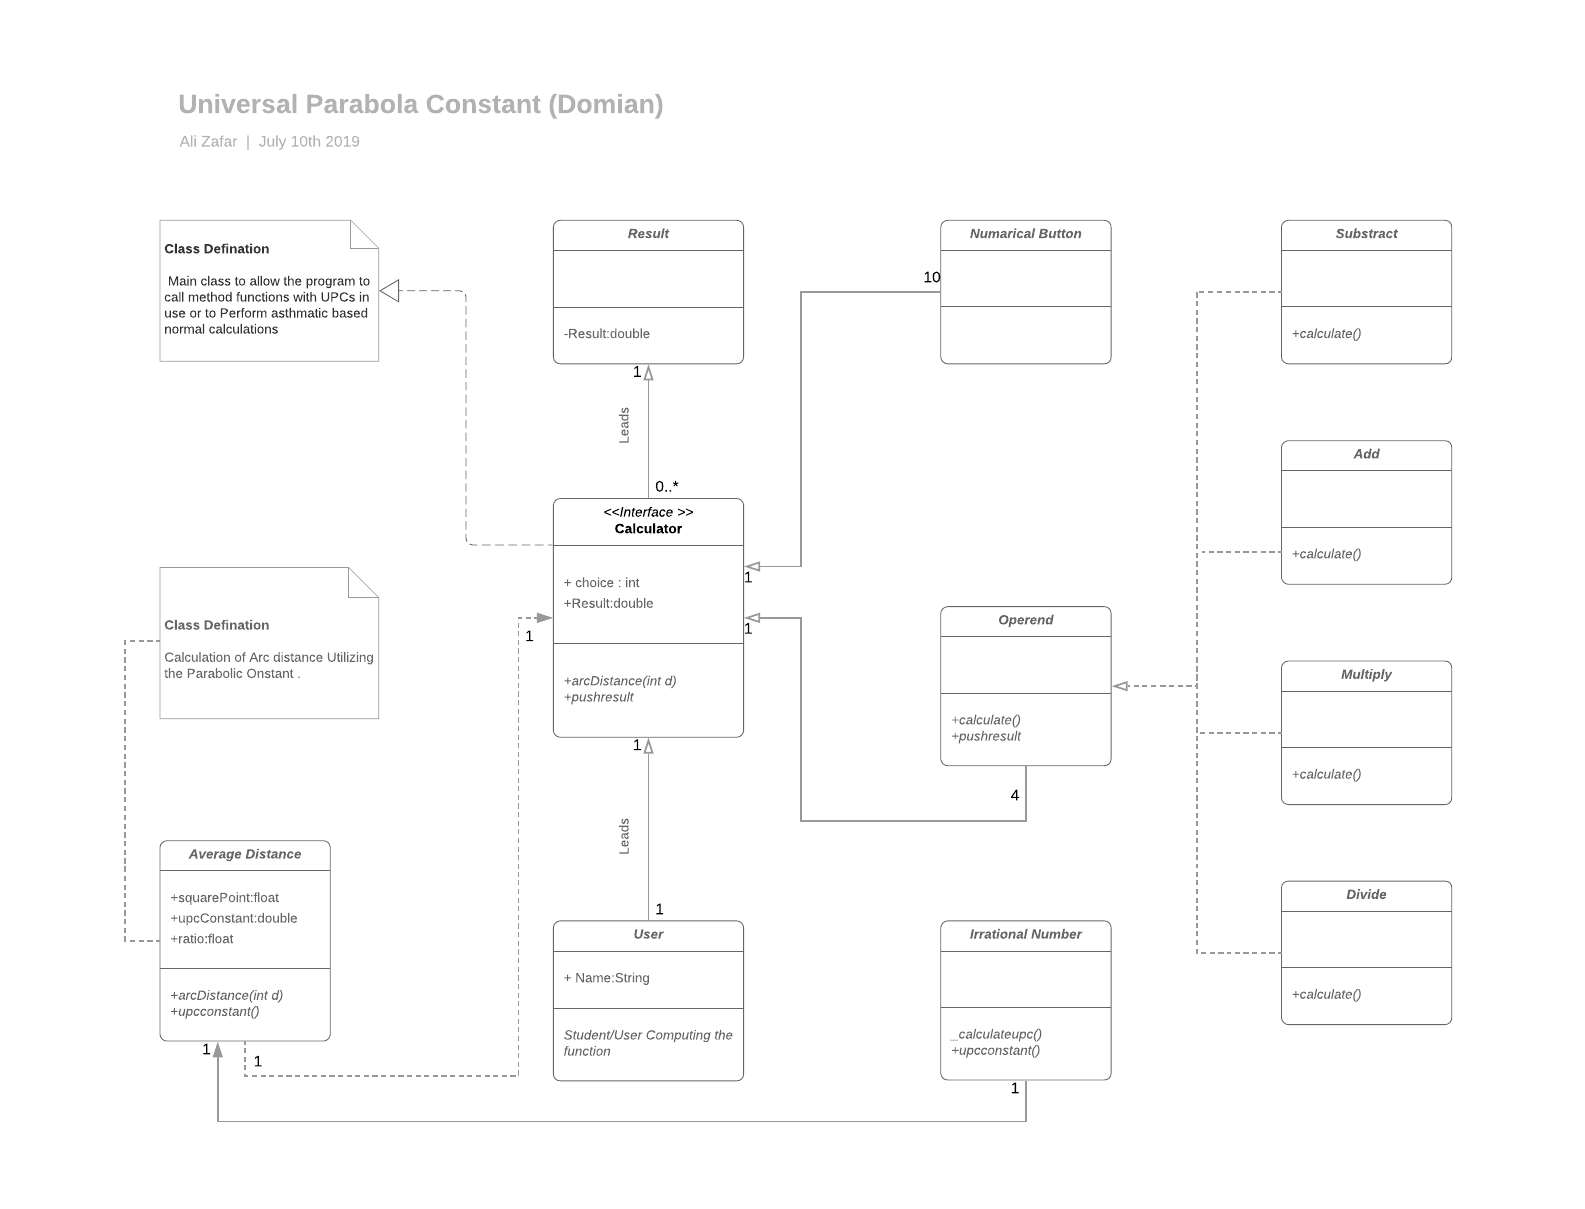
\includegraphics[width=\textwidth]{Assets/Domain.png}
     \caption{Domain Modal for the UPC Calculator}
     \label{fig:my_label}
     \hfill\newline
     \textbf{Concept Explanations }\hfill\break\\
     \begin{enumerate}
        
         \item \textbf{Calculator} : Main class  to allow the program to  call method functions with UPC(Universal Parabolic Constant) in use  or to Perform asthmatic based normal calculations  
         \item \textbf{Operend} : Used as a father class for all asthmatic operands operands can be responsible for a different task. For example, addition is one of the operands which responsible for adding the value, subtraction is also one of the operands which responsible for subtracting the value etc
         \item \textbf{Digital Number} : A set of numerical constants from 0 to 9
         \item \textbf{Irrational Number} : It is the class where the primary constant (Universal parabolic constant) is calculated. 
         \item \textbf{Average Distance} : Calculation of Arc distance Utilizing the Parabolic Constant .
         
     \end{enumerate}
 \end{figure}
 
 
 
 
 
 \begin{figure}
 \section{Activity Diagram}
     \centering{
     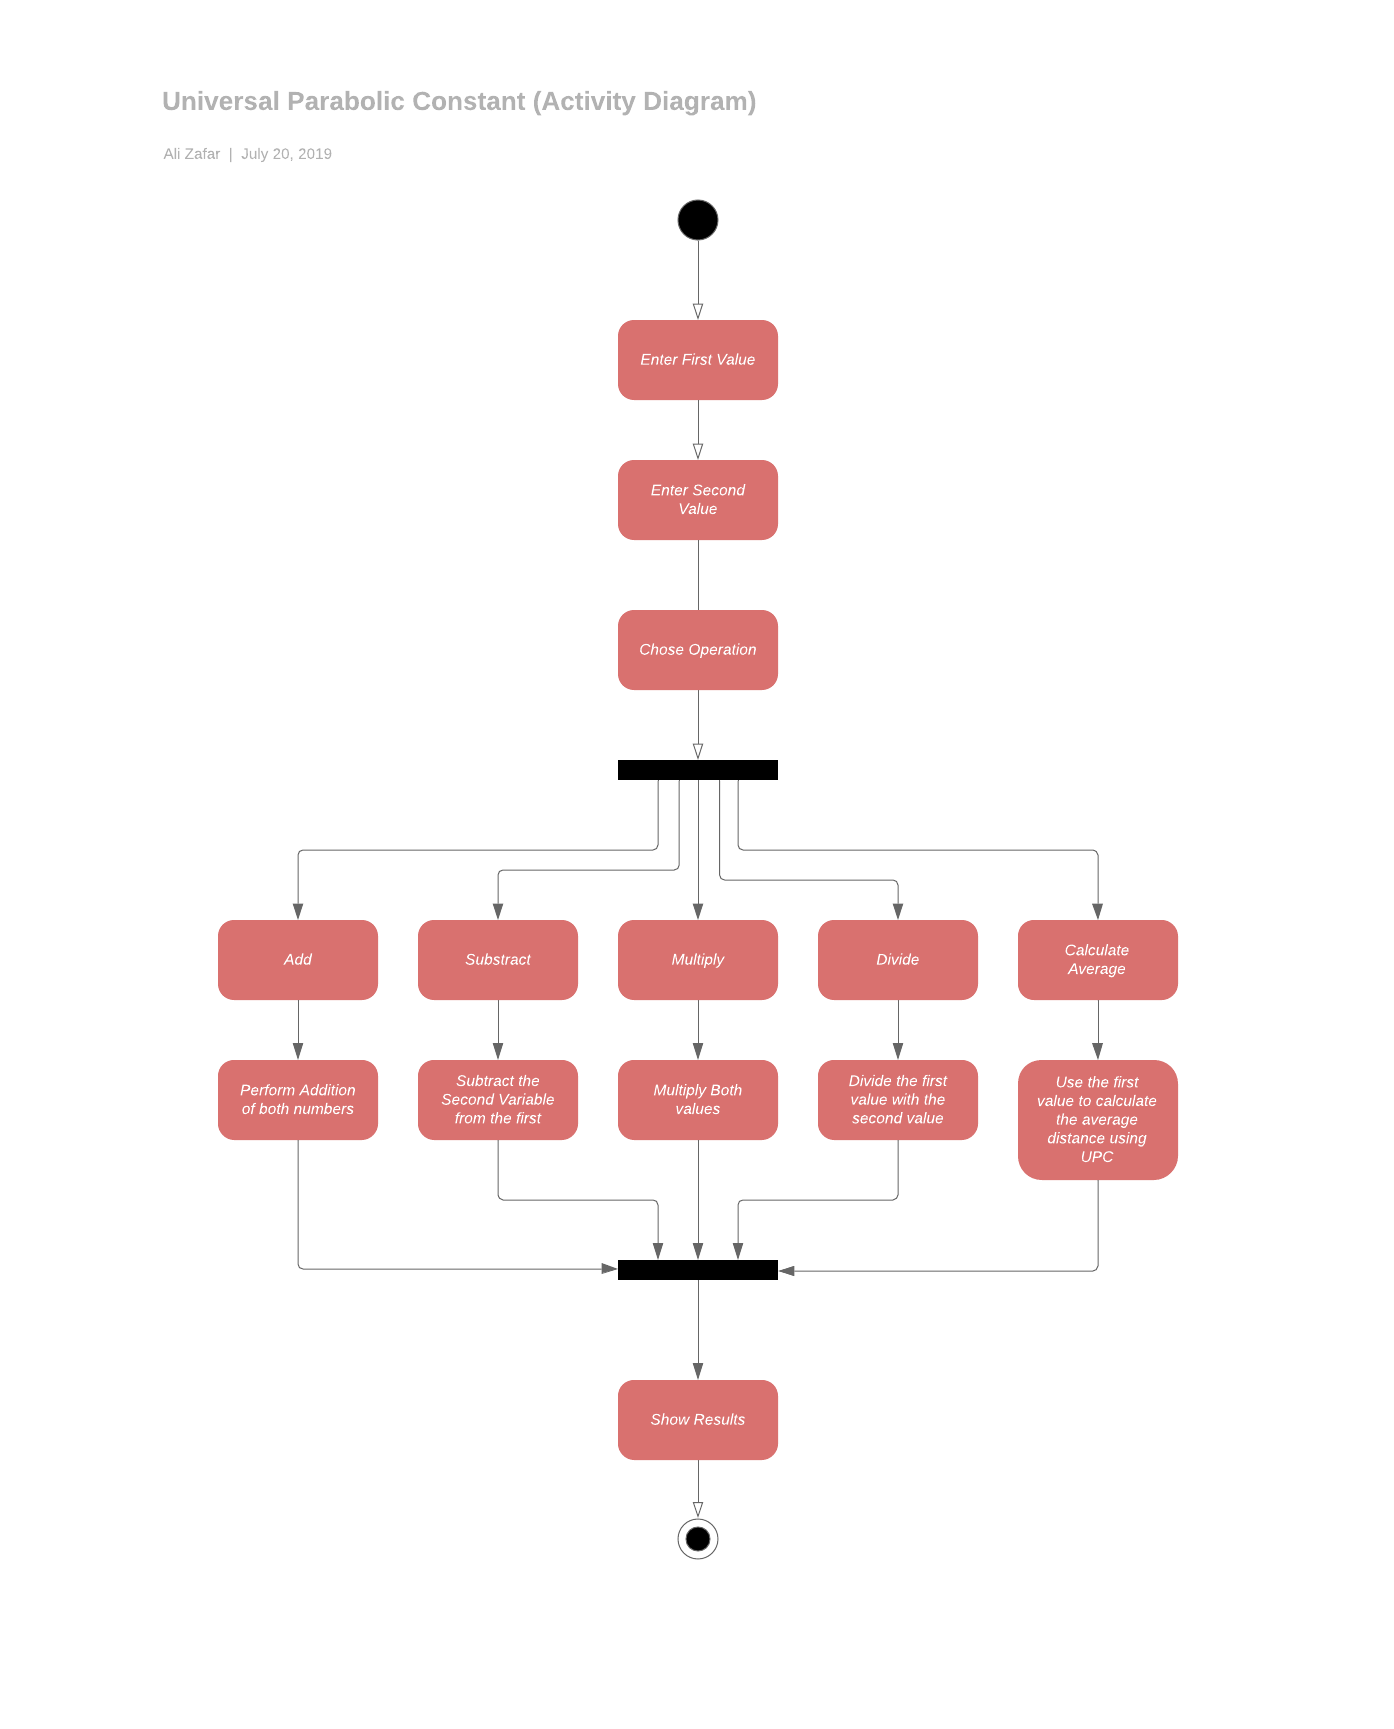
\includegraphics[scale=0.6]{Assets/Activity.png}
     \caption{Activity Diagram for the UPC Calculator}
     \label{fig:my_label}}}
     
        \subsection{Flow Explanation}
 After Initiating the start of the program the user is asked to enter the numbers they want to calculate, and chose the particular operand they want to do the calculation with, or calculate the average distance from the parabola using the Utilizing the Universal Parabolic Constant function.
        
 \end{figure}
   \begin{figure}
 \section{Use Case Diagram}
     \centering{
     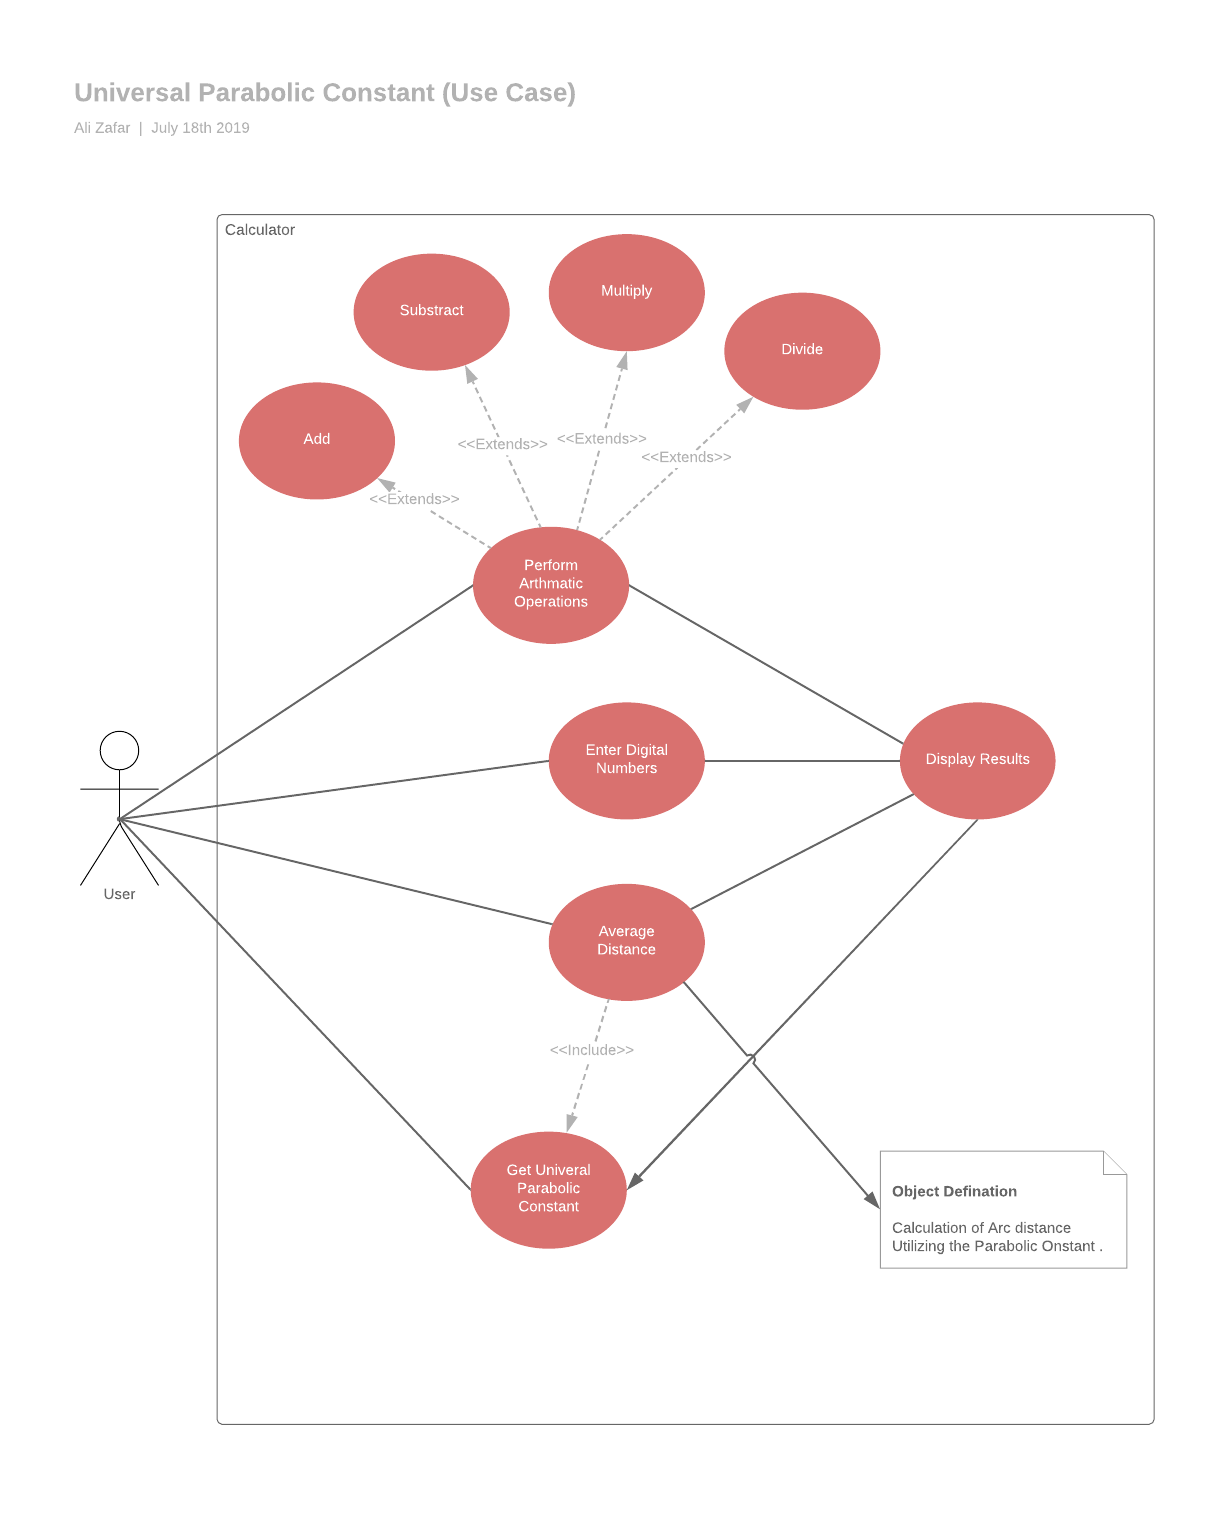
\includegraphics[scale=0.6]{Assets/Usecase.png}
     \caption{Use Case Diagram for the UPC Calculator}
     \label{fig:my_label}}}
      \subsection{Use Case Explanation}
     \begin{enumerate}
        
         \item \textbf{Perform Arthritic Operations} : Allows the user to select the mathematics operand to perform calculations with the calculator
         \item \textbf{Enter Digital Numbers} : Allows the users to enter numbers to allow the calculator to perform calculations with
         \item \textbf{Average Distance} : Calculation of Arc distance Utilizing the Parabolic Constant .
        \item \textbf{Get Parabolic Constant} : Calculate the parabolic constant and show as output or utilize in another function.  
     \end{enumerate}

 \end{figure}

 











\newpage
\chapter{References}
\begin{quote}
    

\begin{enumerate}
\item  {\it Universal parabolic constant\/} www.revolvy.com/page/Universal-parabolic-constant?cr=1,2005).
\item Nick Babich, The Art of the User Interview, {medium.springboard.com/the-art-of-the-user-interview-cf40d1ca62e8 , Oct 9, 2017}
\item  {\it Universal parabolic constant Wolfram Analysis\\}   
http://mathworld.wolfram.com/UniversalParabolicConstant.html.
\end{enumerate}


        

\end{quote}



\end{document}



















